% !TEX root = ./main.tex
\documentclass[a4paper]{article}
% Course language: use [english] or [german].
\usepackage[german]{ajnotes}
\title{\textbf{Mikrooekonomik — Teil 6}}
\begin{document}
    \maketitle
    % Attach the given problem sheet: drop it in this folder as sheet.pdf and
    % un-comment the next line (pdfpages is already loaded by the preamble).
     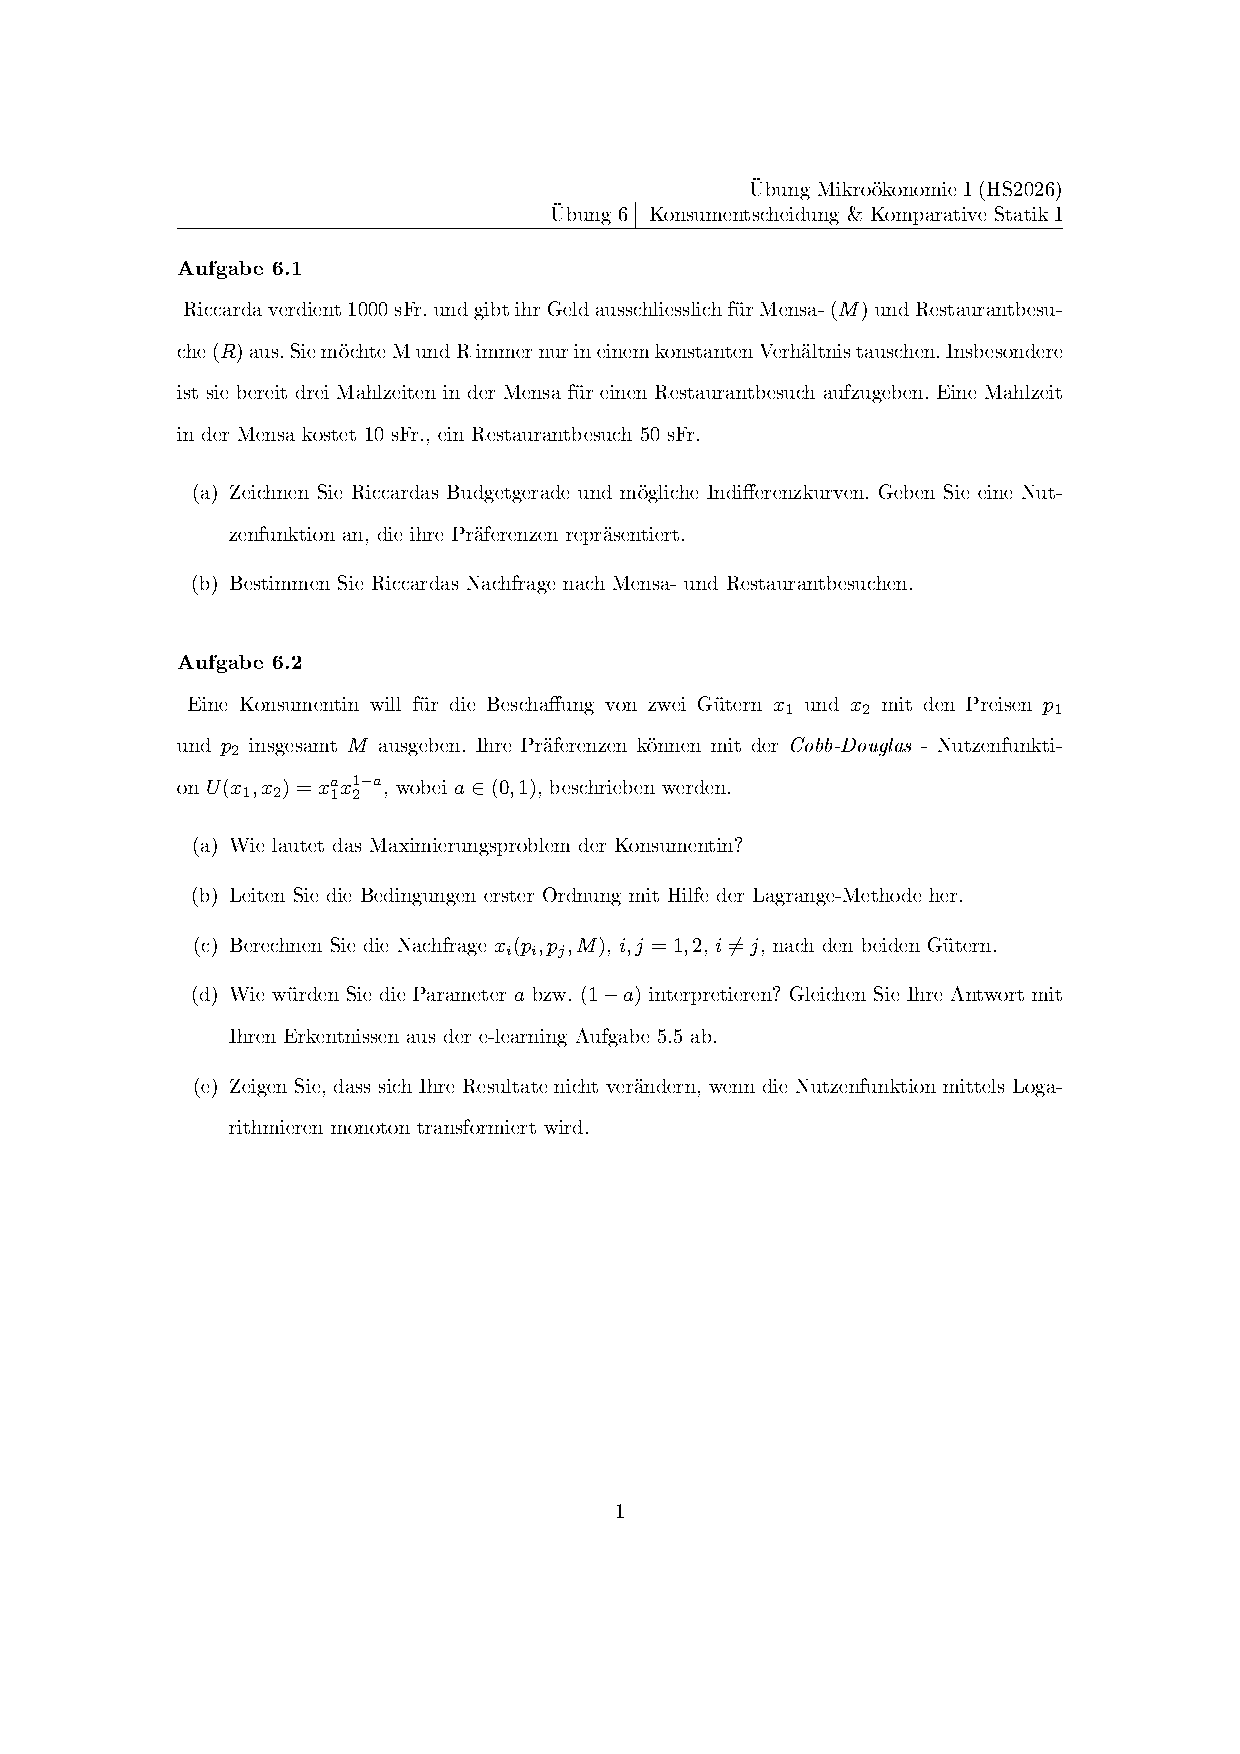
\includepdf[pages=-]{sheet.pdf}
    \exercise{6.1}
    \begin{itemize}
        \item M = 1000, Pr = 50, Pm = 10
        \item U(M,R) = M +3R (Weil Perfekte Substitute sind, ist Nutzenfunktion Linear wie Budgetgerade und nicht konvex)
        \item Extrempunkte $(R_max = 1000/50 und M_max 1000/10) $
    \end{itemize}
    \subexercise{b}
    \begin{itemize}
        \item Nachfrage wird anhand von 
    \end{itemize}
    
    \exercise{6.2}
    \subexercise{a}
    Nutzenfunktion wird anhand der Budgetbedingung maximiert.
    \subexercise{d}
    Parameter sind ein mass für den Anteil des Budgets, die den jeweiligen Güter für sich nach den Präferenzen des Subjekts ansprechen
    Bei Cobb-Douglas Funktionen können immer die Einkommensanteile pro Gut anhand der Exponenten berechnet werden in Form (a*M/Px).

    

\end{document}
